\documentclass[twocolumn]{article}    % two-column because cheat sheets fit like that
\usepackage{preamble}
\newcommand\coursename{Astrodynamics}

\begin{document}
\section*{Midterm}
\RaggedRight
\footnotesize 
\setlength{\tabcolsep}{11pt}
\begin{table}[b]
    \centering
    \footnotesize
    \begin{tabular}{lcccc}
        \toprule
        \textbf{Quantity} & \textbf{Circular} & \textbf{Elliptical} & \textbf{Parabolic} & \textbf{Hyperbolic} \\
        \midrule
        Parametric equation & \(x^2 + y^2 = r^2\) & \(x^2/a^2 + y^2/b^2 =1\) & \(x^2 = 2py\) & \(x^2/a^2 - y^2/b^2 =1\)\\
        Eccentricity & \(e=0\) & \(e = \sqrt{a^2-b^2}/a \quad 0<e<1\)& \(e= 1\) &  \(e=\sqrt{a^2+b^2/a^2} \quad e>1\) \\
        Perifocal distance & \(q=a\) &  \(q=a(1-e)\) & \(q=p/2\) &\(q=a(1-e)\)\\
        Mean angular motion & \(n = \sqrt{\mu/|a|^3}\) & \(n = \sqrt{\mu/|a|^3}\) & \(n=\sqrt{\mu}\) &\(n = \sqrt{\mu/|a|^3}\)\\
        Period & \(T=2\pi/n\) & \(T=2\pi/n\) & \(T=\infty\) & \(T=\infty\)\\
        Anomaly & \(f = M = E\) & \(\tan\left(\frac{f}{2}\right) = \sqrt{\frac{1+e}{1-e}}\tan\left(\frac{E}{2} \right)\) & \(\tan\left(\frac{f}{2} \right) =\frac{D}{\sqrt{2q}}\) & \(\tan\left(\frac{f}{2}\right) = \sqrt{\frac{e+1}{e-1}} \tanh\left(\frac{H}{2} \right)\)\\
        Mean anomaly & \(M = M_0 + nt\) & \(M = E-e\sin E\) & \(M = qD + D^3/6\) & \(M = e\sinh H - H\)\\
        Radius (from focus) & \(r=a\) & \(r = a(1-e\cos E)\) & \(r=q + D^2/2\) & \(r = a(1-e\cosh H)\)\\
        Range rate & \(r\dot{r} = 0\) & \(r\dot{r} = e\sqrt{a\mu} \sin E\) & \(r\dot{r} = \sqrt{\mu}D\) & \(r\dot{r} = e\sqrt{|a|\mu}\sinh H\)\\
        % Areal velocity & \(d A/dt = \sqrt{a\mu}/2\) & \(dA/dt = \sqrt{a\mu(1-e^2)}/2\) & \(dA/dt = \sqrt{\mu q/2}\) & \(dA/dt = \sqrt{a\mu(1-e^2)}/2\)\\
        Specific total orbit energy & \(\varepsilon<0\) & \(\varepsilon<0\) & \(\varepsilon=0\) & \(\varepsilon >0\) \\
        \bottomrule
    \end{tabular}
\end{table}


\begin{equation*}
    \frac{d}{dt} \left( \prescript{\mathcal{B}}{}{}{\bm{r}} \right)_{\mathcal{N}} = \frac{d}{dt}\left( \prescript{\mathcal{B}}{}{\bm{r}} \right)_{\mathcal{B}} + \prescript{\mathcal{B}}{}{\bm{\omega}}_{\mathcal{B}/\mathcal{N}} \times \prescript{\mathcal{B}}{}{\bm{r}} \hspace{30pt} \bm{v} = \bm{\omega} \times \bm{r}
\end{equation*}
\begin{equation*}
    \prescript{\mathcal{B}}{}{\bm{\omega}}_{\mathcal{B}/\mathcal{N}}  = \prescript{\mathcal{B}}{}{\bm{\omega}}_{\mathcal{B}} - \prescript{\mathcal{B}}{}{\bm{\omega}}_{\mathcal{N}}      \hspace{30pt} \bm{\omega} = \frac{\bm{r}\times \bm{v}}{r^2}
\end{equation*}
\begin{equation*}
    \begin{bmatrix}
        \prescript{\mathcal{N}}{}{\bm{r}}_{\mathcal{B}} \\ \prescript{\mathcal{N}}{}{\bm{v}}_{\mathcal{B}} 
    \end{bmatrix} = \begin{bmatrix}
        \prescript{\mathcal{N}}{\mathcal{B}}{\bm{R}} & \bm{0}\\
        \prescript{\mathcal{N}}{\mathcal{B}}{\bm{R}} \left[\prescript{\mathcal{B}}{}{\bm{\omega}}_{\mathcal{B}/\mathcal{N}} \times \right] & \prescript{\mathcal{B}}{}{\bm{\omega}}_{\mathcal{B}/\mathcal{N}} 
    \end{bmatrix} \begin{bmatrix}
        \prescript{\mathcal{B}}{}{\bm{r}}_{\mathcal{B}} \\ \prescript{\mathcal{B}}{}{\bm{v}}_{\mathcal{B}} 
    \end{bmatrix}
\end{equation*}
\begin{equation*}
     \left[\prescript{\mathcal{B}}{}{\bm{\omega}}_{\mathcal{B}/\mathcal{N}} \times \right] = \begin{bmatrix}
        0 & -\omega_3 & \omega_2\\ 
        \omega_3 & 0 & -\omega_1 \\
        -\omega_2 & \omega_1 & 0
    \end{bmatrix} \impliedby \prescript{\mathcal{B}}{}{\bm{\omega}}_{\mathcal{B}/\mathcal{N}} =\begin{bmatrix}
        \omega_1 \\ \omega_2 \\ \omega_3
    \end{bmatrix}
\end{equation*}
\begin{equation*}
    r = \frac{p}{1+e\cos f} \hspace{30pt}  \dot{r} = \frac{r^2\dot{f} e \sin f}{p} \hspace{30pt} p = a(1-e^2) = \frac{h^2}{\mu} 
\end{equation*}
\begin{equation*}
    a = \frac{r_p+r_a}{2} \hspace{30pt} e = \frac{r_a-r_p}{r_a+r_p} \hspace{30pt} b = a\sqrt{1-e^2}
\end{equation*}
\begin{equation*}
     n = \frac{h}{a^2 \sqrt{1-e^2}} = \frac{2\pi}{T} \hspace{25pt}   M_{\operatorname{later}} = n \Delta t + M_{\operatorname{now}} \hspace{25pt} v_{\operatorname{esc}} = \sqrt{\frac{2\mu}{r}}
\end{equation*}
\begin{equation*}
    M = E - \sin E \hspace{30pt} M = e \sinh H - H \hspace{30pt} T^2 = 4\pi^2a^3/\mu
\end{equation*}
\begin{equation*}
    \frac{v^2}{2} -\frac{\mu}{r} = \varepsilon \hspace{30pt} \varepsilon = -\frac{\mu}{2a} \hspace{30pt} G \approx 6.67 \times 10^{-11}\, \frac{\text{m}^3}{\text{kg}\cdot \text{s}^2} 
\end{equation*}
\begin{equation*}
    \text{\underline{{2-Body}}: }\ddot{\bm{r}} = -\frac{\mu}{r^3}\bm{r} \hspace{30pt} \underline{N\text{-Body}}:\, \ddot{\bm{R}}_i = G\sum_{j=1,\, \neq i}^N \frac{m_j}{r_{ij}^3}\bm{r}_{ij} 
\end{equation*}
\begin{equation*}
     r_{SOI\text{ of } m_2} = r_{21} \left( \frac{m_2}{m_3}\right)^{2/5} \hspace{5pt}\text{For } m_3>m_2 >>m_1
\end{equation*}
\begin{equation*}
    \begin{matrix}
        \text{For hyperbolics }\\ (\textit{ie, }a<0,\, e> 1)     
    \end{matrix}
    \begin{cases}
        \begin{matrix}
        x = a(e- \cosh H)\\y = a\sqrt{e^2-1} \sinh H    
    \end{matrix} &
    % \hspace{30pt}
    \begin{matrix}
        f_\infty = \pm \operatorname{acos} -e^{-1}\\
        \delta = \pm 2 \operatorname{asin} e^{-1}
    \end{matrix}
    \end{cases}
\end{equation*}
\begin{equation*}
    I_{sp} =\frac{v_e}{g_0} = \frac{T}{\dot{m} g_0} \hspace{30pt}  \text{\underline{Rocket eq.}: }\Delta v = v_e \ln \left(\frac{m_0}{m_f} \right)  
\end{equation*}
\begin{equation*}
    \text{\underline{Hohmann transfer}: } \Delta v_A = |v_{T,\,p} - v_1|, \hspace{5pt} \Delta v_B = |v_2 - v_{T,\,a}|
\end{equation*}

% \subsection*{Frames}
\begin{itemize}
    \item \textbf{Cylindrical}, \(\mathcal{C}\): \(\{\hat{c}_d,\, \hat{c}_\theta,\, \hat{c}_z\}\), \(\prescript{\mathcal{C}}{}{\bm{r}} = d\hat{c}_d + z \hat{c}_z\),\\ \(\theta = \operatorname{acos}\left(\frac{\hat{u}_x \cdot \bm{r}_{xy}}{d}\right)\), \(\prescript{\mathcal{C}}{\mathcal{U}}{R} = \bm{R}_z(\theta)\)
    \item \textbf{Spherical}, \(\mathcal{S}\): \(\{\hat{s}_r,\, \hat{s}_\theta,\,\hat{s}_\phi\}\), \(\prescript{\mathcal{S}}{}{\bm{r}} = r\hat{s}_r\), \(\theta = \operatorname{acos}\left( \frac{\hat{u}_x\cdot \bm{r}_{xy}}{\|\bm{r}_{xy}\|}\right)\),\\ \(\phi = \operatorname{acos}\left( \frac{\hat{u}_z\cdot \bm{r}_z}{r} \right)\), \(\prescript{\mathcal{S}}{\mathcal{U}}{\bm{R}} = \bm{R}_y(\phi)\bm{R}_z(\theta)\)
    \item \textbf{Earth-Centered Inertial} (ECI), \(\mathcal{I}\)
    \begin{equation*}
        \{\hat{i}_x,\, \hat{i}_y,\, \hat{i}_z\} = \{\text{First point of Ares},\,   \hat{i}_z \times \hat{i}_x,\, \text{True North pole} \}
    \end{equation*}
    
    \item \textbf{Earth-Centered Earth-Fixed} (ECEF), \(\mathcal{E}\)
    \begin{equation*}
        \{\hat{e}_x,\, \hat{e}_y,\, \hat{e}_z\} = \{\text{Greenwich meridian},\,  \hat{e}_z \times \hat{e}_x ,\, \text{True North Pole}\}
    \end{equation*}
    \begin{equation*}
        \text{LST} = \text{GMST} + \text{Long.} \iff \gamma(t) = \gamma_G(t) + \lambda \hspace{19pt}        \prescript{\mathcal{E}}{\mathcal{I}}{\bm{R}} =\bm{R}_z(\gamma_G(t)) 
    \end{equation*}
    % \begin{equation*}
    %     \prescript{\mathcal{E}}{\mathcal{I}}{\bm{R}} =\begin{bmatrix}
    %         \cos \gamma_G(t) & \sin \gamma_G(t)  & 0\\
    %         -\sin \gamma_G(t) & \cos \gamma_G(t)  & 0\\
    %         0&0&1
    %     \end{bmatrix}
    % \end{equation*}

    \item \textbf{Topocentric} (some combo of up, east, north), \(\mathcal{T}\)

    

    \item \textbf{Perifocal} \(\mathcal{P}:\,\{\hat{i}_e,\, \hat{i}_p,\, \hat{i}_h\} = \{\text{Ecc.},\, \text{Parameter},\, \text{out-of-plane}\}\)
    \begin{equation*}
        \text{Motion confined to plane, so } \bm{r} = x\hat{i}_e + y\hat{i}_p = r\cos f \hat{i}_e + r\sin f\hat{i}_p
    \end{equation*}

    \item \textbf{Orbit}, \(\mathcal{O}: \, \{\hat{i}_r,\, \hat{i}_\theta,\, \hat{i}_h \}\), \textbf{Velocity}, \(\mathcal{V}: \, \{\hat{v}_r,\, \hat{v}_n,\, \hat{v}_h \}\), \(\prescript{\mathcal{V}}{\mathcal{O}}{\bm{R}} =\bm{R}_z(\beta) \)
    \begin{equation*}
         \bm{h} = \bm{r} \times \bm{v} = r^2 \dot{f} \hat{i}_h \hspace{18pt} \bm{\omega}_{\mathcal{O}/\mathcal{P}} = \dot{f} \hat{i}_h \hspace{18pt} \bm{v} = (he\sin f)/p \hat{v}_r + h/r\hat{v}_\theta
    \end{equation*}
    % \begin{equation*}
    %     \prescript{\mathcal{V}}{\mathcal{O}}{\bm{R}} =\begin{bmatrix}
    %         \cos \beta & \sin \beta & 0\\
    %         -\sin\beta & \cos\beta & 0\\
    %         0&0&1
    %     \end{bmatrix}
    % \end{equation*}



    \item \textbf{3D Orientation} \text{\oe} \(= \begin{bmatrix}
        a & e & i & \Omega & \omega & (f \text{ XOR } M_0)
    \end{bmatrix}^T\)
    \begin{equation*}
        \prescript{\mathcal{P}}{\mathcal{I}}{\bm{R}} = \bm{R}_z(\omega) \bm{R}_x(i) \bm{R}_z(\Omega) = \begin{bmatrix}
            \hat{i}_e & \hat{i}_p & \hat{i}_h
        \end{bmatrix}  \hspace{20pt} i = \operatorname{acos}(\prescript{\mathcal{P}}{\mathcal{I}}{\bm{R}}[3,\,3] )
    \end{equation*}
    \begin{equation*}
             \Omega = \operatorname{atan}\left( \frac{\prescript{\mathcal{P}}{\mathcal{I}}{\bm{R}}[3,\,1]}{-\prescript{\mathcal{P}}{\mathcal{I}}{\bm{R}}[3,\,2]}\right) \hspace{30pt} \omega = \operatorname{atan} \left( \frac{\prescript{\mathcal{P}}{\mathcal{I}}{\bm{R}}[1,\,3]}{\prescript{\mathcal{P}}{\mathcal{I}}{\bm{R}}[2,\,3]}\right)
    \end{equation*}    
\end{itemize}

\newpage
\begin{figure}[h]
    \centering
    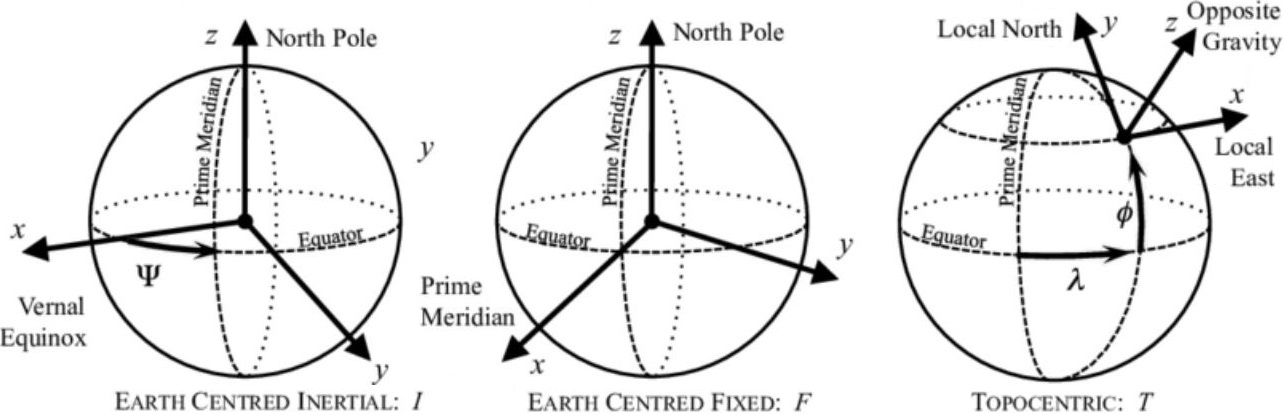
\includegraphics[width=\linewidth]{figures/topocentric_frames.jpg}
\end{figure}
\begin{figure}[h]
    \centering
    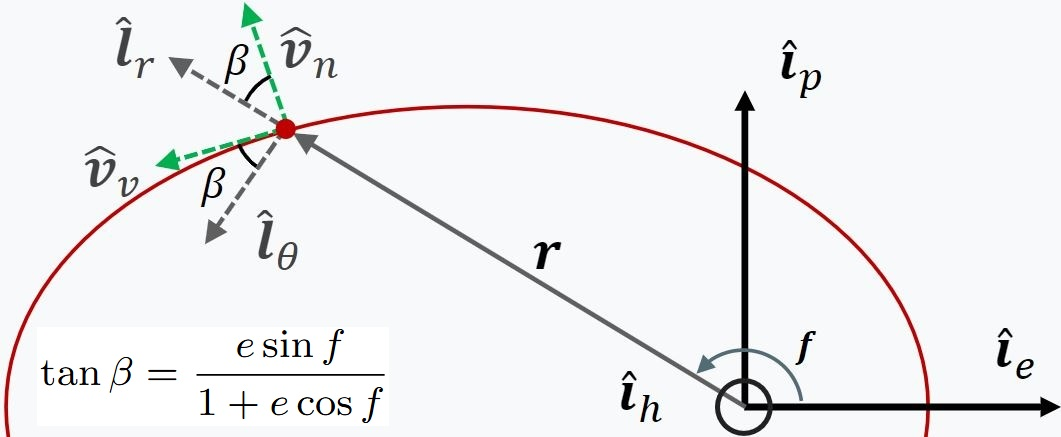
\includegraphics[width=0.85\linewidth]{figures/orbit_frames_smaller.jpg}
\end{figure}

\begin{figure}[h!]
    \centering
    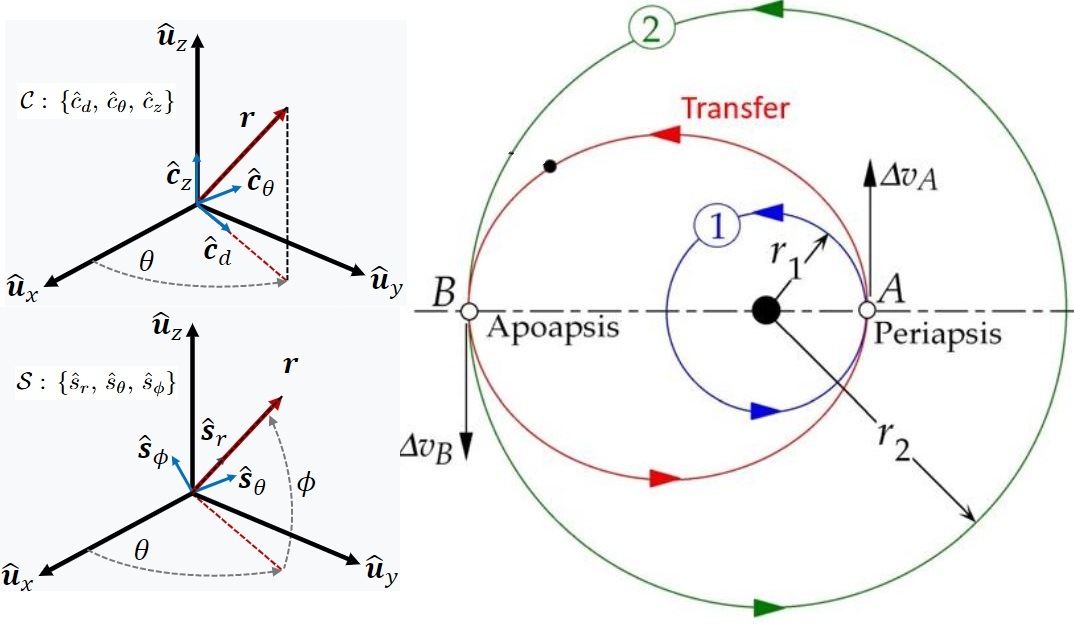
\includegraphics[width=\linewidth]{figures/combo_figure.jpg}
\end{figure}

    
\begin{figure}[h!]
    \centering
    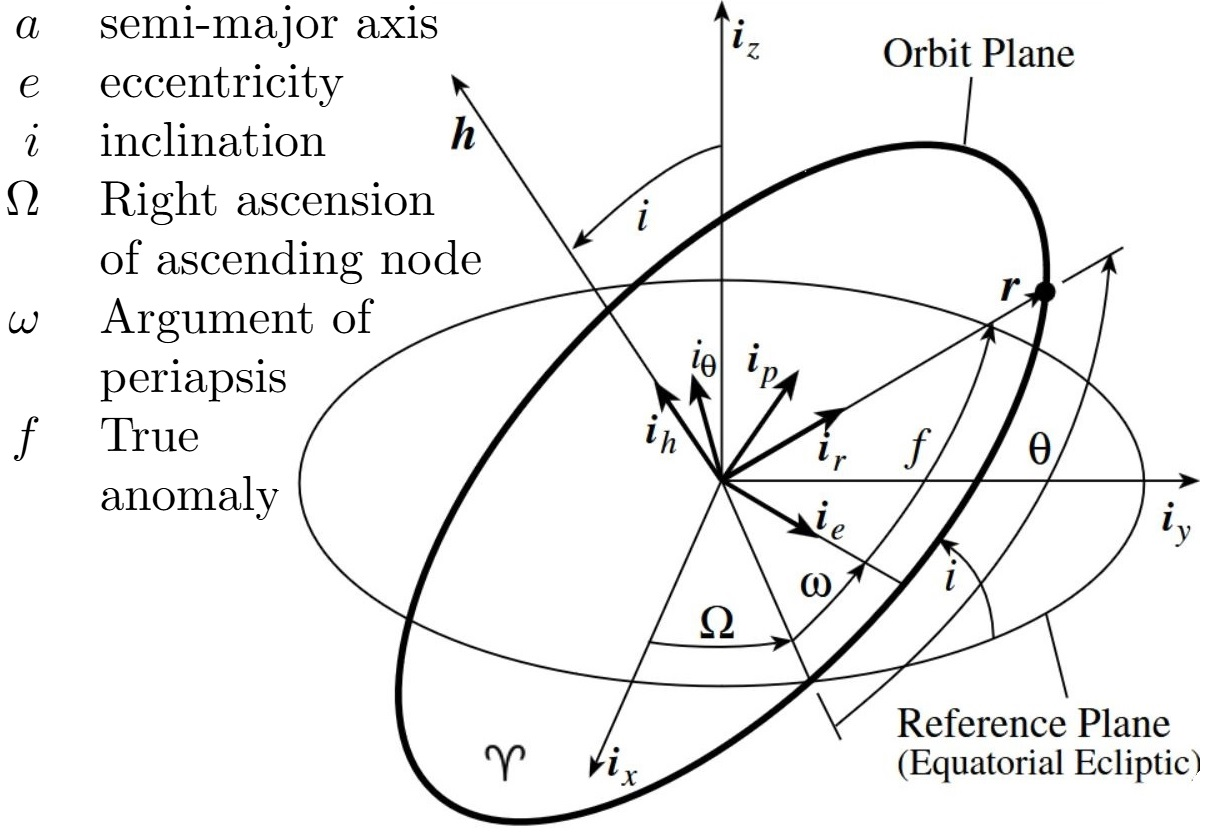
\includegraphics[width=0.9\linewidth]{figures/classical_orbital_elements_diagram.jpg}
\end{figure}


% \vspace{3in}




\newpage
\subsection*{Conversions}
\begin{itemize}
    \item Cartesian to Classical
    \begin{enumerate}
        \item \(v_r = \bm{v} \cdot \hat{r}\), \(v_\perp^2 = v^2 - v_r^2\)
        \item \(\bm{h} = \bm{r} \times \bm{v}\)
        \item \(i = \operatorname{acos}(\bm{h}_z / h)\), \(\bm{N} = \hat{k} \times \bm{h}\)
        \item \(\Omega = \operatorname{acos}(\bm{N}_x/N) \text{ if } \bm{N}_y \geq0 \text{ else }2\pi -\operatorname{acos}(\bm{N}_x/N)\)
        \item \(\bm{e} = (\bm{v}\times \bm{h})/\mu\)
        \item \(p = h^2/\mu\), \(a = p/(1-e^2)\)
        \item \(\omega = \operatorname{acos}(\frac{\bm{e}\cdot \bm{N}}{eN}) \text{ if } \bm{e}_z\geq0 \text{ else } 2\pi - \operatorname{acos}(\frac{\bm{e}\cdot \bm{N}}{eN})\)
        \item \(f = \operatorname{acos} (\frac{\bm{e}\cdot\bm{r}}{er}) \text{ if } v_r\geq 0 \text{ else }2\pi - \operatorname{acos} (\frac{\bm{e}\cdot\bm{r}}{er})\)
    \end{enumerate}
    Note: This should be updated to instead use \(\prescript{\mathcal{P}}{\mathcal{I}}{\bm{R}}\) method for extracting angles.

    % \newpage
    \item Classical to Cartesian
    \begin{enumerate}
        \item \(p = a(1-e^2\), \(r= p/(1+e\cos f)\), \(h = \sqrt{\mu p}\)
        \item \(\dot{f} = h/r^2\), \(\dot{r} = (h e \sin f) /p\)
        \item Assemble state in Perifocal, and rotate to Inertial
        \begin{equation*}
            \prescript{\mathcal{P}}{}{\bm{x}} = \begin{bmatrix}
                r \cos f \\ r \sin f \\ 0\\ 
                -r \dot{f} \sin f + \dot{r} \cos f \\
                r \dot{f} \cos f + \dot{r} \sin f\\
                0
            \end{bmatrix} \hspace{20pt} \prescript{\mathcal{I}}{}{\bm{x}} = \begin{bmatrix}
                \prescript{\mathcal{I}}{\mathcal{P}}{\bm{R}} & \bm{0}\\ \bm{0} & \prescript{\mathcal{I}}{\mathcal{P}}{\bm{R}}
            \end{bmatrix} \prescript{\mathcal{P}}{}{\bm{x}}
        \end{equation*}
    \end{enumerate}
\end{itemize}

% \newpage
\subsection*{Kepler's Laws}
\begin{enumerate}
    \item The orbit of a planet is an ellipse with the Sun at one of the two foci.
    \item A line segment joining a planet and the Sun sweeps out equal areas during equal intervals of time.
    \item The square of a planet's orbital period is proportional to the cube of the length of the semi-major axis of its orbit \(T^2 = 4\pi^2a^3/\mu\). 
\end{enumerate}
\begin{figure}[!ht]
    \centering
    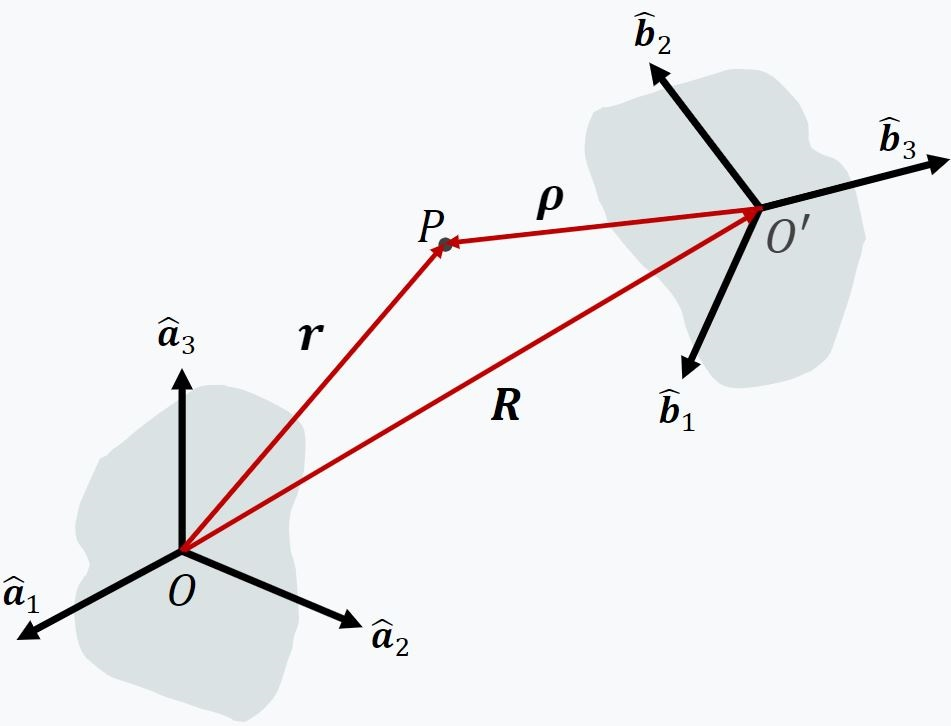
\includegraphics[width=0.5\linewidth]{figures/hw1_prob10_diagram.jpg}
    \caption{Two frames in motion. Source: Lecture 1, slide 17.}
    \label{fig:problem10_diagram}
\end{figure}
In relation to the frames depicted in Fig.~\ref{fig:problem10_diagram}, and beginning from the following expression for the velocity of point  \(P\)
\begin{equation*}
    (\bm{v}_P)_\mathcal{A} = (\bm{v}_{O'})_\mathcal{A} +  (\bm{v}_P)_\mathcal{B} + \bm{\omega}_{\mathcal{B}/\mathcal{A}} \times \bm{\rho}
\end{equation*}
the acceleration of point \(P\), \((\bm{a}_P)_\mathcal{A}\), is found by application of the Transport Theorem, presented here by example
\begin{equation*}
    \text{Transport Theorem: } \hspace{30pt} \frac{d}{dt} (\prescript{\mathcal{E}}{}{\bm{r}}_\mathcal{N}) = \frac{d}{dt} (\prescript{\mathcal{E}}{}{\bm{r}}_\mathcal{E}) + \bm{\omega}_{\mathcal{E}/\mathcal{N}} \times \prescript{\mathcal{E}}{}{\bm{r}} 
\end{equation*}
and is 
\begin{align*}
    (\bm{a}_P)_\mathcal{A} =& \frac{d}{dt}(\prescript{\mathcal{A}}{}{\bm{v}_{O'}})_\mathcal{A} + \frac{d}{dt}(\prescript{\mathcal{B}}{}{\bm{v}}_P)_\mathcal{B} + \bm{\omega}_{\mathcal{B}/\mathcal{A}} \times \prescript{\mathcal{B}}{}{\bm{v}}_P + \frac{d}{dt}\bm{\omega}_{\mathcal{B}/\mathcal{A}} \times \bm{\rho} + \bm{\omega}_{\mathcal{B}/\mathcal{A}} \times  \frac{d}{dt}\bm{\rho} \\
    =& (\prescript{\mathcal{A}}{}{\bm{a}_{O'}})_\mathcal{A} + (\prescript{\mathcal{B}}{}{\bm{a}}_P)_\mathcal{B} + \bm{\omega}_{\mathcal{B}/\mathcal{A}} \times \prescript{\mathcal{B}}{}{\bm{v}}_P + \bm{\alpha}_{\mathcal{B}/\mathcal{A}} \times \bm{\rho} + \bm{\omega}_{\mathcal{B}/\mathcal{A}} \times \left( (\prescript{\mathcal{B}}{}{\bm{v}}_P) + \bm{\omega}_{\mathcal{B}/\mathcal{A}}\times\bm{\rho} \right)\\
    =& \boxed{(\prescript{\mathcal{A}}{}{\bm{a}_{O'}})_\mathcal{A} + (\prescript{\mathcal{B}}{}{\bm{a}}_P)_\mathcal{B} + 2\bm{\omega}_{\mathcal{B}/\mathcal{A}} \times \prescript{\mathcal{B}}{}{\bm{v}}_P + \bm{\alpha}_{\mathcal{B}/\mathcal{A}} \times \bm{\rho} + \bm{\omega}_{\mathcal{B}/\mathcal{A}} \times \bm{\omega}_{\mathcal{B}/\mathcal{A}}\times\bm{\rho} = (\bm{a}_P)_\mathcal{A} }
\end{align*}
with the following names for each term:
\begin{itemize}
    \item Linear acceleration of frame \(O'\):  \((\prescript{\mathcal{A}}{}{\bm{a}_{O'}})_\mathcal{A}\) 
    \item Linear acceleration of point \(P\) in frame \(\mathcal{B}\): \((\prescript{\mathcal{B}}{}{\bm{a}}_P)_\mathcal{B}\)
    \item Coriolis acceleration: \(2\bm{\omega}_{\mathcal{B}/\mathcal{A}} \times \prescript{\mathcal{B}}{}{\bm{v}}_P \)
    \item Euler acceleration: \(\bm{\alpha}_{\mathcal{B}/\mathcal{A}} \times \bm{\rho} \)
    \item Centrifugal acceleration: \(\bm{\omega}_{\mathcal{B}/\mathcal{A}} \times \bm{\omega}_{\mathcal{B}/\mathcal{A}}\times\bm{\rho}\)
\end{itemize}








\end{document}